\selectlanguage{ngerman}%
\frenchspacing%
\begin{ledgroupsized}[r]{120mm}%
\footnotesize%
\pstart%
\noindent\textbf{Überlieferung:}%
\pend%
\end{ledgroupsized}%
\begin{ledgroupsized}[r]{114mm}%
\footnotesize%
\pstart%
\parindent -6mm%
\makebox[6mm][l]{\textit{L}}%
Konzept:
LH~XXXV~10,\;13 Bl.\;7.
Ein Zettel (etwa 9,5~x~20~cm);
Ränder beschnitten, zum Teil unregelmäßig.
Zwei vollbeschriebene Seiten.
\pend
\end{ledgroupsized}
\selectlanguage{latin}
\frenchspacing
\vspace{8mm}
\pstart%
\normalsize%
\noindent%
\lbrack%
\href{\Scan{LH_35_10_13_007r}}%
{7\,r\textsuperscript{o}}%
\rbrack%
\hfill%
\edlabel{LH_35_10_13_007r_titel-1}
\textls{Casus eccentrici concursus simplicissimus}
\indexS{concursus eccentricus}%
\indexS{casus simplex}%
\hfill%
\phantom{\lbrack7\,r\textsuperscript{o}\rbrack}%
\edtext{}{%
\xxref{LH_35_10_13_007r_titel-1}{LH_35_10_13_007r_titel-2}%
\lemma{\textit{Neben der Überschrift:}}\Afootnote{%
Hic satis videor accessisse.}
\lemma{\textit{Quer am Rand, nachträglich:}}\Afootnote{%
Examinemus%
\textsuperscript{\lbrack a\rbrack}
quid fiat in vi mortua%
\indexS{vis mortua}
seu conatu nascente,%
\indexS{conatus nascens}
ut si in aqua%
\indexS{aqua}
\textit{AB} sit gravis,%
\indexS{corpus grave}
\textit{LM} levis tantundem.%
\indexS{corpus leve}%
\pagelabel{LH_35_10_13_007r_rndbmrk_1}%
\\[1.5ex]%
{\footnotesize%
\textsuperscript{\lbrack a\rbrack}~%
Examinemus:
Siehe N.\;\ref{60107},
\refpassage{LH_35_10_13_008r_kehg-1}{LH_35_10_13_008r_kehg-2}.%
}%
}}
\pend%
\pstart%
\noindent%
\centering%
Scheda 1.\indexS{scheda}
\quad%
\edlabel{LH_35_10_13_007_007r_datum-1}%
Septemb.\;691 \textlangle--\textrangle%
\edlabel{LH_35_10_13_007r_titel-2}
\pend%
\vspace{1.0em}%
\pstart%
\noindent%
Si in plano paginae\indexS{planum paginae}\indexS{pagina}
concurrant rectae parallelae aequales \textit{AB}, \textit{LM}%
\indexS{rectae parallelae concurrentes}
celeritate aequali,\indexS{celeritas concursus}
concursu eccentrico directo%
\indexS{concursus eccentricus}%
\indexS{concursus directus}%
\lbrack,\rbrack\
quaeritur quid contingat.
Et sane si partes respondentes \textit{BC} et \textit{LN} %
sint infinite parvae,\indexS{pars infinite parva}
reflexio est nulla,\indexS{reflexio nulla}
si sint aequales toti,
reflexio est totalis;\indexS{reflexio totalis}
et neutro modo admista est
\edtext{%
gyratio.\indexS{gyratio admixta}
Si partes \textit{BC}, \textit{LN} sint admodum parvae,
fiet aliqua progressio\indexS{progressio ab utraque parte}
ab utraque parte,
et proinde
concursus et\indexS{concursus corporum}
gyratio progredientium,\indexS{gyratio corporum progredientium}%
}{%
\lemma{gyratio.}\Bfootnote{%
\textit{(1)}~Itaque
\textit{(2)}~Si vero \textit{BC} et \textit{LN} sint minores totis, mista erit p
\textit{(3)}~Si partes %
\lbrack...\rbrack\ et proinde
\bars{concursus et \textit{erg.}}
gyratio progredientium,%
~\textit{L}}}
sine qua progressio amborum
(\protect\vphantom)%
par enim utriusque ratio est%
\protect\vphantom()
intelligi non potest.%
\pend%
\vspace{2.5em} %
\centerline{%
\includegraphics[width=0.74\textwidth]{%
gesamttex/edit_VIII-4/images/LH_35_10_13_007_d1_007r.pdf%
}}
\vspace{1.0em}
\centerline{%
\lbrack\textit{Fig.\:1}\rbrack%
}
\newpage%
\pstart%
Gyratio\indexS{gyratio circa punctum}
fiet circa aliquod punctum%
\indexS{punctum gyrationis}
ut \textit{D} vel \textit{P},
ut scilicet puncta \textit{B} et \textit{L} reflectantur%
\lbrack,\rbrack\
\textit{A} et \textit{M} procedant.
\edtext{%
Punctum ut \textit{D} an sit%
}{%
\lemma{Punctum}\Bfootnote{%
\bars{ut \textit{D}
\bars{vel \textit{P} \textit{gestr.}}
\textit{erg.}}
an sit%
~\textit{L}}}
medium inter \textit{A} et \textit{B},
an vero inter \textit{A} et \textit{C},
dispiciendum
\edlabel{35_10_13_007r_1a}%
est.%
\edtext{}{%
\xxref{35_10_13_007r_1a}{35_10_13_007r_1b}%
\lemma{est.}\Bfootnote{%
\textit{(1)}~Videndum etiam an non detur casus
\textit{(2)}~\lbrack/\rbrack\ Quoniam autem datur progressus
\textit{(a)}~sine ref
\textit{(b)}~merus, datur reflexio m
\textit{(c)}~merus si
\textit{BC} nulla,
\bars{sed \textit{erg.}}
datur regressus %
\lbrack...\rbrack\ dari medium,%
~\textit{L}}}%
\pend
\pstart
Quoniam autem datur progressus merus%
\indexS{progressus merus}
si
\textit{BC} nulla,
sed datur regressus merus%
\indexS{regressus merus}
si \textit{BC} tota;
sequitur casum dari medium,%
\indexS{casus medius}%
\edlabel{35_10_13_007r_1b}
ubi nec est progressus\indexS{progressus in concursu eccentrico}
nec regressus concurrentium,\indexS{regressus in concursu eccentrico}
sed mera gyratio\indexS{gyratio corporum in concursu}%
\lbrack,\rbrack\
quod videtur contingere
cum \textit{BC} est media totius,
seu cum rectae concurrunt
\edlabel{35_10_13_007r_2a}%
medietatibus seu cum
$BC = BE$
(\protect\vphantom)%
adeoque et
$LN = LQ$%
\protect\vphantom().%
\edtext{}{%
\xxref{35_10_13_007r_2a}{35_10_13_007r_2b}%
\lemma{medietatibus}\Bfootnote{%
\textit{(1)}~. Datur et
\textit{(2)}~. Ubi vero
\textit{(3)}~seu cum %
\lbrack...\rbrack\ et $LN = LQ$\protect\vphantom().
\textit{(a)}~Cum \textit{BC} est minor
\textit{(aa)}~\textlangle seq\textrangle\
\textit{(bb)}~\textit{BE} \textlangle er\textrangle\
\textit{(b)}~Cum vero %
\lbrack...\rbrack\ minor quam 
\bars{\textit{LN ändert Hrsg.}}, erit%
~\textit{L}}}
Cum vero \textit{BC} est minor quam
\lbrack\textit{BE}\rbrack,
erit%
\edlabel{35_10_13_007r_2b}
regressus\indexS{regressus mixtus gyrationi}
gyrationi mistus,%
\indexS{gyratio mixta regressui}
et oportet locum esse %
\edlabel{35_10_13_007r_5a}%
ubi vis respectiva\indexS{vis respectiva}
seu vis ictus\indexS{vis ictus}
sit aeque divisa in gyrationem et regressum.%
\indexS{vis divisa in gyrationem et regressum}
\edtext{}{%
\xxref{35_10_13_007r_5a}{35_10_13_007r_5b}%
\lemma{ubi}\Bfootnote{%
\textit{(1)}~vis sit aeque divisa in respectivam et in
\textit{(2)}~vis respectiva %
\lbrack...\rbrack\ et regressum.
\lbrack/\rbrack\
\textit{(a)}~Ubicunque gyratio et progressus simul fiunt, ut fit cum \textit{BC} est paulo major quam \textit{BE}, oportet gyrationem esse progressu celeriorem, alioqui impedirentur (\protect\vphantom)quod si fiunt, oportet gyrationem esse \lbrack/\rbrack\
\textit{(b)}~Dispiciendum est, an
\bars{hic \textit{erg.}}
simul fieri %
\lbrack...\rbrack\ et progressus.%
~\textit{L}}}
\pend%
\pstart%
Dispiciendum est,
an hic simul fieri possint
gyratio\indexS{gyratio mixta progressui}
et progressus.\indexS{progressus mixtus gyrationi}%
\edlabel{35_10_13_007r_5b}%
\edtext{}{%
\lemma{\textit{Quer am Rand, nachträglich:}}%
\applabel{FnA:35_10_13_007r_navis}%
\Afootnote{%
Res reducta videtur ad hanc considerationem,%
\indexS{consideratio}
ut \textit{AC} et \textit{BC} se praetereuntes
contrariis directionibus aggelascant.%
\textsuperscript{\lbrack a\rbrack}
\newline%
\hspace*{7.6mm}%
Notandum in concursu Eccentrico\indexS{concursus eccentricus}
vim ictus\indexS{vis ictus}
non coincidere cum vi respectiva\indexS{vis respectiva}
et vim ictus\indexS{vis ictus}
esse tantum partium centrice concurrentium.%
\indexS{partes concurrentes centrice}
Ut ergo regressus\indexS{regressus in concursu eccentrico}
a vi ictus\indexS{vis ictus}%
\textsuperscript{\lbrack b\rbrack}
cum progressu\indexS{progressus conciliatus cum regressu}
reliquae partis concilietur%
\lbrack,\rbrack\
sola circulatione\indexS{circulatio in concursu eccentrico}
effici potest.
Vis ictus in%
\textsuperscript{\lbrack c\rbrack}
unum corporum%
\lbrack,\rbrack\
seu dimidium totius ictus\indexS{ictus}%
\lbrack,\rbrack\
est dimidium potentiae circulationis%
\indexS{potentia circulationis}%
\textsuperscript{\lbrack d\rbrack}
si potentia circulandi\indexS{potentia circulandi} est debilior.
Sin minus%
\lbrack,\rbrack\
vis ictus\indexS{vis ictus}
quam patitur unum corpus
est id quod restat
vi circulationis%
\indexS{vis circulationis}
detracta a respectiva.%
\indexS{vis respectiva}
Reliquum potentiae respectivae\indexS{potentia respectiva}
est vis progressus.\indexS{vis progressus}
Videndum
an hic tuta motuum compositio.\indexS{compositio motuum}
Sane in navi\indexS{navis} succedit:
Ita et hic videtur.
Est enim ac si quid in navi\indexS{navis}
circuletur.
{\footnotesize%
\\[1.5ex]%
\textsuperscript{\lbrack a\rbrack}~%
aggelascant: Die Anspielung bezieht sich wohl auf das Diagramm \lbrack\textit{Fig.\:2}\rbrack.
\quad
\textsuperscript{\lbrack b\rbrack}~%
ictus
\textit{(1)}~et
\textit{(2)}~cum%
~\textit{L}
\quad
\textsuperscript{\lbrack c\rbrack}~%
in unum %
\lbrack...\rbrack\ totius ictus
\textit{erg.\;L}
\quad
\textsuperscript{\lbrack d\rbrack}~%
circulationis
\textit{(1)}~\textlangle residuum dimidia\textrangle\
\textit{(2)}~\textlangle si \textendash\textrangle\
\textit{(3)}~si potentia %
\lbrack...\rbrack\ Sin minus
\textit{(a)}~residuum est dimid
\textit{(b)}~vis ictus
\textit{(aa)}~\textlangle est i\textrangle\
\textit{(bb)}~quam patitur
\lbrack...\rbrack\ a respectiva.%
~\textit{L}
}%
}}
\lbrack%
\href{\Scan{LH_35_10_13_007v}}%
{7\,v\textsuperscript{o}}%
\rbrack%
\pend%
\newpage%
\vspace*{0.0em}%
\centerline{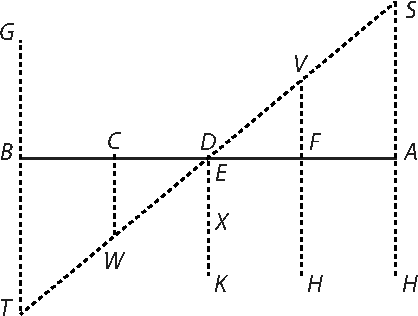
\includegraphics[width=0.46\textwidth]{gesamttex/edit_VIII-4/images/LH_35_10_13_007_d2_007v.pdf}}
\vspace{1.0em}
\centerline{\lbrack\textit{Fig.\:2}\rbrack}
\vspace{1.5em}
\pstart%
\noindent%
Poterit res eo reduci,
ut
\edtext{%
concipiamus totam \textit{AB}
habere vim priorem,%
\indexS{vis prior}
sed \textit{BC} habere regrediendi conatum,%
\indexS{conatus regrediendi}
ast \textit{AC} conatum progrediendi.%
\indexS{conatus progrediendi}%
}{%
\lemma{concipiamus}\Bfootnote{%
\textit{(1)}~\textit{BC} et \textit{CA} habere conatum
\textit{(2)}~totam quidem
\textit{(a)}~\textit{BC}
\textit{(b)}~\textit{AB} habere vim respectivam, sed \textit{BC} tantum vim regrediendi
\textit{(3)}~totam \textit{AB} %
\lbrack...\rbrack\ \textit{BC} habere
\textit{(a)}~vim
\textit{(b)}~regrediendi conatum,
\textit{(aa)}~sed
\textit{(bb)}~ast \textit{AC} conatum progrediendi.%
~\textit{L}}}%
\pend%
\vspace{0.5em}%
\pstart%
\noindent%
\lbrack%
\textit{Nachfolgend kleingedruckter Text in L gestrichen:}\rbrack%
\pend%
\vspace{0.5em}%
\footnotesize%
\pstart%
\noindent%
\edtext{%
Et per hunc%
}{%
\lemma{Et}\Bfootnote{%
\textit{(1)}~quia
\textit{(2)}~\bars{ne \textit{streicht Hrsg.}}
\textit{(3)}~per hunc%
~\textit{L}}}
regrediendi conatum%
\indexS{conatus regrediendi}
sumatur ipsius \textit{AC} pars \textit{AF}
\edtext{%
aequalis%
\lbrack,\rbrack\
similis et similiter
posita ipsi \textit{BC},%
}{%
\lemma{aequalis}\Bfootnote{%
\textit{(1)}~et
\textit{(2)}~similis et similiter posita
\textit{(a)}~ipsi \textit{BF}
\textit{(b)}~ipsi \textit{BC},%
~\textit{L}}}
patet eas compensari inter
\edtext{se,
dum}{%
\lemma{se,}\Bfootnote{%
\textit{(1)}~at
\textit{(2)}~dum%
~\textit{L}}}
ambae gyrantur circa \textit{E}.
Et hactenus totam \textit{BC} habere suum
\edlabel{35_10_13_007v_6a}%
progressum.%
\indexS{progressus in concursu eccentrico}
\edtext{}{%
\xxref{35_10_13_007v_6a}{35_10_13_007v_6b}%
\lemma{progressum}\Bfootnote{%
\lbrack/\rbrack\
\textit{(1)}~An
\textit{(2)}~Ergo dicemus
\textit{(a)}~circulationem nasci qualis
\textit{(b)}~regressum
\textit{(aa)}~in circulatione sci
\textit{(bb)}~nasci tantum quantus est conatus
\textit{(aaa)}~ipsius \textit{BC}
\textit{(bbb)}~regrediendi in %
\lbrack...\rbrack\ quantitatem circulationis,%
~\textit{L}}}%
\pend%
\normalsize%
\vspace{0.5em}%
\pstart%
\noindent%
Ergo dicemus regressum\indexS{regressus in concursu eccentrico}
nasci tantum
quantus est conatus regrediendi%
\indexS{conatus regrediendi}
in \textit{BC},
quod determinat quantitatem circulationis,%
\indexS{quantitas circulationis}%
\edlabel{35_10_13_007v_6b}
nam est eius quantitas
\edtext{dimidia.
Adeoque}{%
\lemma{dimidia}\Bfootnote{%
\textit{(1)}~, sed
\textit{(2)}~. Adeoque%
~\textit{L}}}
circulationi impenditur\indexS{circulatio in concursu eccentrico}
tam conatus regrediendi\indexS{conatus regrediendi}
quem habet \textit{BC} per ictum,\indexS{ictus}
quam conatus progrediendi\indexS{conatus progrediendi}
quem habet \textit{AF} per
\edlabel{35_10_13_007v_4a}%
se.%
\edtext{}{%
\xxref{35_10_13_007v_4a}{35_10_13_007v_4b}%
\lemma{se.}\Bfootnote{%
\textit{(1)}~Itaque
\textit{(2)}~Sed
\textit{(a)}~absoluto conatui progrediendi
\textit{(b)}~absolutae progressioni impenditur conatus progrediendi%
~\textit{L}}}
Sed absolutae progressioni%
\indexS{progressio absoluta}
impenditur conatus progrediendi%
\indexS{conatus progrediendi}%
\edlabel{35_10_13_007v_4b}
ipsius \textit{CF}.
Ubi jam notandum
\edtext{%
est progressionem in circulatione sumi%
\indexS{progressio sumta in circulationem}%
\indexS{circulatio in concursu eccentrico}
ductis velocitatibus in puncta mota.%
\indexS{velocitas ducta in punctum motum}%
\indexS{punctum motum}%
}{%
\lemma{est}\Bfootnote{%
\textit{(1)}~contum circulati
\textit{(2)}~progressionem in circulatione sumi
\textit{(a)}~in ratione
\textit{(b)}~ductis velocitatibus in puncta mota.%
~\textit{L}}}
\pend%
\pstart%
Perinde autem res sese habet,
ac
\edtext{%
si in unam aggelascere ponamus tres rectas,
nempe%
}{%
\lemma{si}\Bfootnote{%
\textit{(1)}~\textlangle cum\textrangle\
\textit{(2)}~simul
\textit{(3)}~\textlangle cum\textrangle\
\textit{(4)}~congelascere ponamus tres rect
\textit{(5)}~in unam %
\lbrack...\rbrack\ tres rectas,
\bars{nempe \textit{erg.}}%
\textit{L}}}
\textit{BC} habentem conatum $\overline{BC \cdot G},$
et ei aequalem \textit{AF}
habentem conatum contrarium\indexS{conatus contrarius}
$\overline{AF\cdot H},$
et denique \textit{FC} habentem conatum \textit{EK},
ubi non alius obtineri potest
\edtext{%
exitus\indexS{exitus}%
\lbrack,\rbrack\
quo
scilicet nihil amittatur
potentiae,\indexS{potentia amissa}%
}{%
\lemma{exitus}\Bfootnote{%
\textit{(1)}~nihil amittendo
\textit{(2)}~quo scilicet nihil amittatur potentiae,%
~\textit{L}}}
quam ut circulatio fiat circa \textit{E},%
\indexS{circulatio circa punctum}
et quidem tanta
ut celeritate\indexS{celeritas circulationis}
ipsius puncti \textit{A} vel \textit{B}
existente \textit{AS},
\edtext{%
\textit{BT}
aequalibus et ad \textit{AB} normalibus,
junctaque \textit{SET} recta%
}{%
\lemma{\textit{BT}}\Bfootnote{%
\textit{(1)}~(\protect\vphantom)aequalibus\protect\vphantom() juncta \textit{SET},
\textit{(2)}~aequalibus et %
\lbrack...\rbrack\ \textit{SET} recta%
~\textit{L}}}
cui ex \textit{F} et \textit{C} eductae normaliter rectae
occurrant in \textit{V} et \textit{W},
sit trapezium \textit{AFVS} vel \textit{BCWT}
aequale\indexS{trapezium}
\edtext{%
rectangulo \textit{FAH} vel \textit{CBG}.%
\indexS{rectangulum}%
}{%
\lemma{rectangulo}\Bfootnote{%
\textit{(1)}~\textit{CBG} vel
\textit{(2)}~\textit{FAH} vel \textit{CBG}.%
~\textit{L}}}
\pend%
\pstart%
Celeritas autem ipsius centri \textit{E}%
\indexS{celeritas centri gravitatis}
erit \textit{EX},
quae quaeritur an sit talis
ut rectang. \textit{AB} in \textit{EX} aequetur
rectangulo \textit{CF} in \textit{DK}.%
\indexS{rectangulum}
\edtext{Ita sane,}{%
\lemma{Ita}\Bfootnote{%
\bars{videtur \textit{gestr.}} sane,%
~\textit{L}}}
nec ita quicquam incommodi orietur
quia quantum ipsi \textit{AF}
absolutae celeritatis additur,%
\indexS{celeritas absoluta}
tantum ipsi \textit{BC}
\edtext{adimitur%
\lbrack,\rbrack\
ita ut in summa}{%
\lemma{adimitur.}\Bfootnote{%
\textit{(1)}~. In eor
\textit{(2)}~ita ut in summa%
~\textit{L}}}
verus motus compositus%
\indexS{motus compositus}
non sit major primo.
Ubi tamen videndum an idem locum habeat,
cum centrum gravitatis%
\indexS{centrum gravitatis}
non est centrum figurae,%
\indexS{centrum figurae}
ubi major quantitas motus additur%
\indexS{quantitas motus addita}
ab una parte quam ab altera
\edtext{adimitur.%
\indexS{quantitas motus ademta}
Immo}{%
\lemma{adimitur.}\Bfootnote{%
\textit{(1)}~Itaque
\textit{(2)}~Immo%
~\textit{L}}}
videndum est
an sufficiat quantitatem motus respici,%
\indexS{quantitas motus servanda}
et an non sit opus
servari virium quantitatem.%
\indexS{quantitas virium servanda}
Atque ita est.
Nam et in navi\indexS{navis} servanda est.
Etiam in concurrentibus
vis respectiva servanda est.%
\indexS{vis respectiva servanda}
NB.
\edtext{}%
{\lemma{\textit{Quer am Rand:}}%
\applabel{FnA:35_10_13_007v_navis}%
\Afootnote{%
Quid si sint inaequalia corpora eccentrice concurrentia%
\indexS{concursus eccentricus}%
\indexS{corpora concurrentia inaequalia}%
\indexS{corpora eccentrice concurrentia}%
\lbrack;\rbrack\
faciendus motus reciproce proportionalis,%
\indexS{motus reciproce proportionalis}
ut centrum gravitatis quiescat.%
\indexS{centrum gravitatis quiescens}%
\newline%
\hspace*{7.6mm}
Quid si navem\indexS{navis} hic adhibebimus
ad casus definiendos,\indexS{casus definiendus}
cum centrum gravitatis alias non quiescit.%
\indexS{centrum gravitatis quiescens}%
}}%
\pend%
\selectlanguage{latin}%
\frenchspacing%
\normalsize%
